\section{複雑性の検証実験}

\subsection{概要}

本プロジェクトの目標の要件を満たす戦略表を作成するには、人間が扱いやすいということについて定量的に表し、既存、もしくは新たに作成した戦略表を評価しなければならない。そのため、前期ではコルモゴロフ複雑性を参考にし、連長圧縮を用いることで複雑性を定義し、これをある戦略表を記憶する難易度の評価指標として用いた。しかし、実際に人間がある戦略表を覚える時に感じる難易度と複雑性によって表した難易度は、異なっている可能性がある。そのため、後期では複雑性の検証実験として、いくつかの戦略表を用意し、記憶してもらうという実験を行うことで、複雑性が戦略表を記憶する難易度を正しく表しているかを確かめた。
\bunseki{鳥谷航大}

\subsection{実験の目的}

本実験のもっとも重要な目的は、先述の通り、人間が扱いやすい戦略表というのはどういう戦略表なのかを定量的に表すことである。そのため、本実験では、以下の2つを主な目的とした。
\begin{itemize}
    \item 目的1:本プロジェクトが定義した複雑性が戦略表を記憶する難易度を正しく表しているかを確認すること
    \item 目的2:目的1を達成出来なかった場合、可能な限り戦略表を記憶する難易度を正確に評価できる指標を見つけること
\end{itemize}
目的2について、具体的には、人間のどのような能力がブラックジャックをプレイする能力と関連性を持つかや個人の性格が実験に影響を及ぼすかなどの観点を中心に実験を行った。
\bunseki{鳥谷航大}

\subsection{仮説}

本プロジェクトでは以下の仮説を立て、実験を行った。
\begin{itemize}
    \item 仮説1:複雑性は人間が戦略表を記憶する時に感じる難易度を正確に表すことが出来ない
    \item 仮説2:一般的な認知的判断能力と戦略表を扱う能力は同じ能力、もしくは深い関連性を持つ
    \item 仮説3:リスクを好む・好まない等の性格によって戦略表を記憶し扱う時に違いが生じる
\end{itemize}
それぞれの仮説に対して詳しく説明する。まず仮説1についてであるが、このような仮説を立てた背景として、前期でこの複雑性を用いて性能を評価した時、戦略表の勝率があまり良くない戦略表が高い性能と評価されてしまったことがある。このことから、他に戦略表を記憶する難易度を正確に表すことが出来る指標が存在するのではないか、と考えこのような仮説を立てた。そして、仮説2、仮説3は、先述の他の評価指標として考えられるものである。仮説2は、個人の一般的な認知判断能力が評価指標になるのではないかという仮説である。それに対して、仮説3は、個人のリスクに関する性格が評価指標になるのではないかという仮説である。
\bunseki{鳥谷航大}

\subsection{実験準備}

今回の実験の目的や仮説に合わせ、実験に用いる戦略表や被験者、報酬などは以下のように準備を行った。
まず、今回の実験で用いた戦略表は以下の表\ref{tablea}、表\ref{tableb}、表\ref{tablec}の3つである。
% Please add the following required packages to your document preamble:

\begin{table}[H]
    \caption{戦略表A}
    \label{tablea}
    \begin{center}
        \begin{tabular}{|c|c|c|c|c|c|c|c|c|c|c|c|}
        \hline
        \multicolumn{2}{|c|}{\multirow{2}{*}{}} & \multicolumn{10}{c|}{ディーラーのアップカード}     \\ \cline{3-12} 
        \multicolumn{2}{|c|}{}                  & 2 & 3 & 4 & 5 & 6 & 7 & 8 & 9 & 10 & A \\ \hline
        \multirow{10}{*}{手札の合計}      & 5〜8      & H & H & H & H & H & H & H & H & H  & H \\ \cline{2-12} 
                                    & 9        & H & H & H & H & H & H & H & H & H  & H \\ \cline{2-12} 
                                    & 10       & H & H & H & H & H & H & H & H & H  & H \\ \cline{2-12} 
                                    & 11       & H & H & H & H & H & H & H & H & H  & H \\ \cline{2-12} 
                                    & 12       & H & H & H & H & H & H & H & H & H  & H \\ \cline{2-12} 
                                    & 13       & H & H & H & H & H & H & H & H & H  & H \\ \cline{2-12} 
                                    & 14       & H & H & H & H & H & H & H & H & H  & H \\ \cline{2-12} 
                                    & 15       & H & H & H & H & H & H & H & H & H  & H \\ \cline{2-12} 
                                    & 16       & S & S & S & S & S & S & S & S & S  & S \\ \cline{2-12} 
                                    & 17以上     & S & S & S & S & S & S & S & S & S  & S \\ \hline
        \end{tabular}
    \end{center}
\end{table}

% Please add the following required packages to your document preamble:
% \usepackage{multirow}
\begin{table}[H]
    \begin{center}
    \caption{戦略表B}
    \label{tableb}
    \begin{tabular}{|c|c|c|c|c|c|c|c|c|c|c|c|c|}
    \hline
    \multicolumn{3}{|c|}{\multirow{2}{*}{}}                     & \multicolumn{10}{c|}{ディーラーのアップカード}     \\ \cline{4-13} 
    \multicolumn{3}{|c|}{}                                      & 2 & 3 & 4 & 5 & 6 & 7 & 8 & 9 & 10 & A \\ \hline
    \multirow{28}{*}{手札の合計} & \multirow{9}{*}{ハードハンド}   & 9     & H & H & H & H & H & H & H & H & H  & H \\ \cline{3-13} 
                            &                           & 10    & H & D & D & D & D & H & H & H & H  & H \\ \cline{3-13} 
                            &                           & 11    & D & D & D & D & D & D & D & D & H  & H \\ \cline{3-13} 
                            &                           & 12    & D & D & D & D & D & D & D & D & D  & D \\ \cline{3-13} 
                            &                           & 13    & H & H & S & S & S & H & H & H & H  & H \\ \cline{3-13} 
                            &                           & 14    & S & S & S & S & S & H & H & H & H  & H \\ \cline{3-13} 
                            &                           & 15    & S & S & S & S & S & H & H & H & R  & H \\ \cline{3-13} 
                            &                           & 16    & S & S & S & S & S & H & H & R & R  & R \\ \cline{3-13} 
                            &                           & 17以上  & S & S & S & S & S & S & S & S & S  & S \\ \cline{2-13} 
                            & \multirow{9}{*}{ソフトハンド}   & A,2   & H & H & H & D & D & H & H & H & H  & H \\ \cline{3-13} 
                            &                           & A,3   & H & H & H & D & D & H & H & H & H  & H \\ \cline{3-13} 
                            &                           & A,4   & H & H & D & D & D & H & H & H & H  & H \\ \cline{3-13} 
                            &                           & A,5   & H & H & D & D & D & H & H & H & H  & H \\ \cline{3-13} 
                            &                           & A,6   & H & D & D & D & D & H & H & H & H  & H \\ \cline{3-13} 
                            &                           & A,7   & S & D & D & D & D & S & S & H & H  & H \\ \cline{3-13} 
                            &                           & A,8   & S & S & S & S & S & S & S & S & S  & S \\ \cline{3-13} 
                            &                           & A,9   & S & S & S & S & S & S & S & S & S  & S \\ \cline{3-13} 
                            &                           & A,10  & S & S & S & S & S & S & S & S & S  & S \\ \cline{2-13} 
                            & \multirow{10}{*}{スプリット可能} & A,A   & P & P & P & P & P & P & P & P & P  & P \\ \cline{3-13} 
                            &                           & 2,2   & P & P & P & P & P & P & H & H & H  & H \\ \cline{3-13} 
                            &                           & 3,3   & P & P & P & P & P & P & H & H & H  & H \\ \cline{3-13} 
                            &                           & 4,4   & H & H & H & P & P & H & H & H & H  & H \\ \cline{3-13} 
                            &                           & 5,5   & D & D & D & D & D & D & D & D & H  & H \\ \cline{3-13} 
                            &                           & 6,6   & P & P & P & P & P & H & H & H & H  & H \\ \cline{3-13} 
                            &                           & 7,7   & P & P & P & P & P & P & H & H & H  & H \\ \cline{3-13} 
                            &                           & 8,8   & P & P & P & P & P & P & P & P & P  & P \\ \cline{3-13} 
                            &                           & 9,9   & P & P & P & P & P & S & P & P & S  & S \\ \cline{3-13} 
                            &                           & 10,10 & S & S & S & S & S & S & S & S & S  & S \\ \hline
    \end{tabular}
    \end{center}
\end{table}

% Please add the following required packages to your document preamble:
% \usepackage{multirow}
\begin{table}[H]
    \begin{center}
    \caption{戦略表C}
    \label{tablec}
    \begin{tabular}{|c|c|c|c|c|c|c|c|c|c|c|c|c|}
    \hline
    \multicolumn{3}{|c|}{\multirow{2}{*}{}}                     & \multicolumn{10}{c|}{ディーラーのアップカード}     \\ \cline{4-13} 
    \multicolumn{3}{|c|}{}                                      & 2 & 3 & 4 & 5 & 6 & 7 & 8 & 9 & 10 & A \\ \hline
    \multirow{28}{*}{手札の合計} & \multirow{9}{*}{ハードハンド}   & 9     & H & H & H & H & H & H & H & H & H  & H \\ \cline{3-13} 
                            &                           & 10    & H & D & D & D & D & H & H & H & H  & H \\ \cline{3-13} 
                            &                           & 11    & D & D & D & D & D & D & D & D & H  & H \\ \cline{3-13} 
                            &                           & 12    & D & D & D & D & D & D & D & D & D  & D \\ \cline{3-13} 
                            &                           & 13    & H & H & S & S & S & H & H & H & H  & H \\ \cline{3-13} 
                            &                           & 14    & S & S & S & S & S & H & H & H & H  & H \\ \cline{3-13} 
                            &                           & 15    & S & S & S & S & S & H & H & H & H  & H \\ \cline{3-13} 
                            &                           & 16    & S & S & S & S & S & H & H & H & H  & H \\ \cline{3-13} 
                            &                           & 17以上  & S & S & S & S & S & S & S & S & S  & S \\ \cline{2-13} 
                            & \multirow{9}{*}{ソフトハンド}   & A,2   & H & H & H & H & D & H & H & H & H  & H \\ \cline{3-13} 
                            &                           & A,3   & H & H & H & D & D & H & H & H & H  & H \\ \cline{3-13} 
                            &                           & A,4   & H & H & D & D & D & H & H & H & H  & H \\ \cline{3-13} 
                            &                           & A,5   & H & H & D & D & D & H & H & H & H  & H \\ \cline{3-13} 
                            &                           & A,6   & H & D & D & D & D & H & H & H & H  & H \\ \cline{3-13} 
                            &                           & A,7   & D & D & D & D & D & S & S & H & H  & H \\ \cline{3-13} 
                            &                           & A,8   & S & S & S & S & D & S & S & S & S  & S \\ \cline{3-13} 
                            &                           & A,9   & S & S & S & S & S & S & S & S & S  & S \\ \cline{3-13} 
                            &                           & A,10  & S & S & S & S & S & S & S & S & S  & S \\ \cline{2-13} 
                            & \multirow{10}{*}{スプリット可能} & A,A   & P & P & P & P & P & P & P & P & P  & P \\ \cline{3-13} 
                            &                           & 2,2   & H & H & P & P & P & P & H & H & H  & H \\ \cline{3-13} 
                            &                           & 3,3   & P & P & P & P & P & P & H & H & H  & H \\ \cline{3-13} 
                            &                           & 4,4   & H & H & H & P & P & H & H & H & H  & H \\ \cline{3-13} 
                            &                           & 5,5   & D & D & D & D & D & D & D & D & H  & H \\ \cline{3-13} 
                            &                           & 6,6   & P & P & P & P & P & H & H & H & H  & H \\ \cline{3-13} 
                            &                           & 7,7   & P & P & P & P & P & P & H & H & H  & H \\ \cline{3-13} 
                            &                           & 8,8   & P & P & P & P & P & P & P & P & P  & P \\ \cline{3-13} 
                            &                           & 9,9   & P & P & P & P & P & S & P & P & S  & S \\ \cline{3-13} 
                            &                           & 10,10 & S & S & S & S & S & S & S & S & S  & S \\ \hline
    \end{tabular}
    \end{center}
\end{table}
またこれらの戦略表の複雑性は表\ref{complex}のとおりである。
\begin{table}[H]
    \begin{center}
    \caption{各戦略表の複雑性}
    \label{complex}
    \begin{tabular}{|c|c|c|c|}
        \hline
            & 戦略表A & 戦略表B  & 戦略表B  \\ \hline
        複雑性 & 0.2  & 0.448 & 0.407 \\ \hline
    \end{tabular}   
    \end{center}
\end{table}

次に被験者についてである。被験者は本学の学生から募集をした。募集方法としては、ブラックジャックに関する実験であることや、戦略表を記憶するテストであるなどの実験の内容を事前に知らせずに募集した。募集の結果、男性15人、女性5人の計20人集めることが出来た。被験者の年齢は18〜21歳であった。

今回20人の被験者が集まったため実験時に2つのグループに分けて実験を行った。分けられたグループは記憶する戦略表が異なる。具体的な分け方は以下のとおりである。
\begin{itemize}
    \item グループX:戦略表A、Bを記憶するグループ
    \item グループY:戦略表A、Cを記憶するグループ
\end{itemize}
このようにグループ分けした理由としては、比較的複雑性の低い戦略表Aの成績を確認することで、戦略表Bと戦略表Cの成績の違いの要因が、戦略表の複雑性によってなのか個人差によってなのかを確認するためである。

最後に実験協力の報酬についてである。報酬は実験前に、実験結果の成績に応じて配られるという説明を行い、成績が高い被験者ほど多くの報酬が得られるように分配した。
\bunseki{鳥谷航大}

\subsection{実験の手法・手順}

今回の実験は、異なる複雑性を持つ戦略表を3つ用意し、先述したグループごとに対応する戦略表を記憶してもらった後テストを行うというものである。その後、CRT(Cognitive Reflection Test)やリスク回避性のテストなどを行い、テストの成績との関連性を分析した。詳しい実験手順は以下のとおりである。
\begin{enumerate}
    \item ブラックジャックについての説明を行う
    \item 5〜10分程度の時間を用いて実際にプレイしゲームを理解してもらう
    \item 戦略表を配り10分間で記憶してもらう
    \item テストを配り7分間で回答してもらう
    \item 回答を配り被験者に採点をしてもらいテストを回収する
    \item 4〜6を戦略表を変更しもう一度繰り返す
    \item CRTとリスク回避性のテストについて回答してもらう。回答時間は両方合わせて10〜15分とした。
    \item 結果に応じた報酬を配り実験を終了する
\end{enumerate}
\bunseki{鳥谷航大}

\subsection{実験結果}

今回の実験で得られた主な結果は以下の3つである。
\begin{itemize}
    \item 結果1:テストの成績と複雑性には強い負の相関があること
    \item 結果2:CRTの点数とテストの成績には相関がないこと
    \item 結果3:リスク回避性とテストの成績には相関がないこと
\end{itemize}
ここでは、私達が特に興味深く感じた結果1,2に関して詳しく説明していく。

表\ref{xpoint}がグループXの成績であり、表\ref{ypoint}はグループYの成績である。また、戦略表のテストは満点が30点であり、CRTの満点は11点である。
\begin{table}[H]
    \begin{center}
    \caption{グループXの成績}
    \label{xpoint}
    \begin{tabular}{|c|c|c|c|}
    \hline
         & 戦略表A & 戦略表B  & CRT   \\ \hline
    平均   & 29.1 & 13.8  & 7.2   \\ \hline
    分散   & 2.29 & 12.96 & 3.96  \\ \hline
    標準偏差 & 1.51 & 3.6   & 2.098 \\ \hline
    \end{tabular}
    \end{center}
\end{table}

\begin{table}[H]
    \begin{center}
    \caption{グループYの成績}
    \label{ypoint}
    \begin{tabular}{|c|c|c|c|}
    \hline
         & 戦略表A & 戦略表C  & CRT   \\ \hline
    平均   & 29.8 & 17.5  & 8.8   \\ \hline
    分散   & 0.6  & 2.872 & 1.36  \\ \hline
    標準偏差 & 0.36 & 8.25  & 1.229 \\ \hline
    \end{tabular}
    \end{center}
\end{table}
両方のグループともに、戦略表Aは高い成績となった。そのため、成績とCRT正答率つまり、一般的な認知的判断能力の相関関係を見る時には、戦略表Aから戦略表BまたはCの点数を引いた差とCRT正答率との相関を考えた。図\ref{diffab}がグループXの散布図であり、図\ref{diffac}がグループYの散布図である。
\begin{figure}[H]   
    \begin{center}
        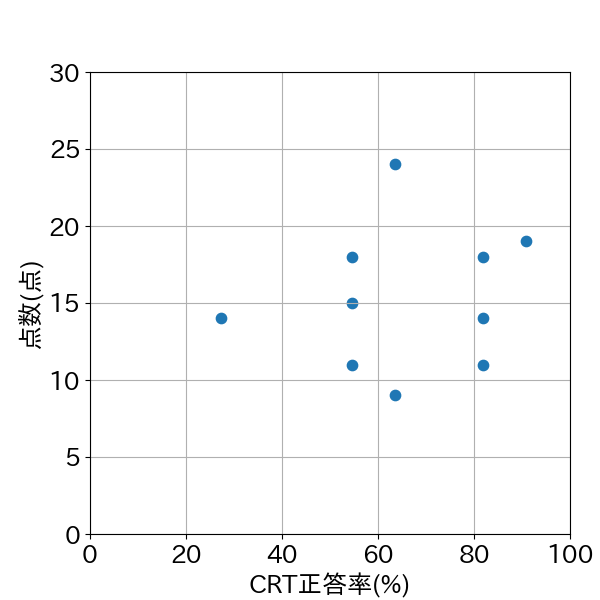
\includegraphics[width=10cm]{figure/experiment-groupX_crt_diffAB.png}
        \caption{CRT正答率と戦略表Aから戦略表Bの点数を引いた値との散布図}
        \label{diffab}
    \end{center}
\end{figure}

\begin{figure}[H]
    \begin{center}
        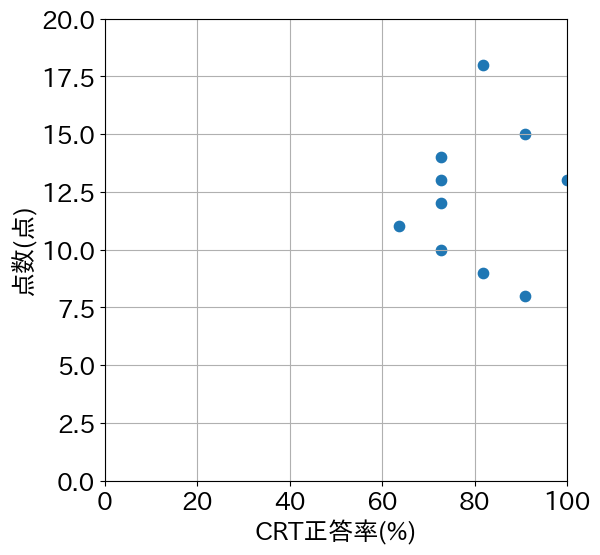
\includegraphics[width=10cm]{figure/experiment-groupY_crt_diffAC.png}
        \caption{CRT正答率と戦略表Aから戦略表Cの点数を引いた値との散布図}
        \label{diffac}
    \end{center}
\end{figure}
また、この散布図より相関係数を求めたところ表\ref{soukan}のようになった。
\begin{table}[H]
    \begin{center}
    \caption{それぞれのグループの相関係数}
    \label{soukan}
    \begin{tabular}{|c|c|c|}
    \hline
                  & グループX & グループY \\ \hline
    CRTと点数の差の相関係数 & 0.145 & 0.079 \\ \hline
    \end{tabular}
    \end{center}
\end{table}
上の表の通り、相関係数は非常に小さいという結果になった。ただし、相関係数が小さくても相関がある可能性があるため、無相関検定を行った。無相関検定の検定条件などは後述の複雑性と成績の相関係数と合わせて詳しく後で述べる。無相関検定の結果、グループX、グループYともに相関が無いことがわかった。

次に、複雑性とテストの成績の関連性についてである。以下の表\ref{average}が各戦略表の複雑性とテストの平均点である。
\begin{table}[H]
    \begin{center}
    \caption{各戦略表の複雑性とテストの平均点}
    \label{average}
    \begin{tabular}{|c|c|c|c|c|}
    \hline
            & 戦略表A(グループX) & 戦略表A(グループY) & 戦略表B  & 戦略表C  \\ \hline
    テストの平均点 & 29.1        & 29.8        & 13.8  & 17.5  \\ \hline
    複雑性     & 0.2         & 0.2         & 0.448 & 0.407 \\ \hline
    \end{tabular}
    \end{center}
\end{table}
さらに、実験で得られたデータを用いて成績と複雑性の相関係数を求めたところ$-0.942$となり、ほぼ$-1$に近い値となった。こちらも無相関検定を行ったところ、非常に強い負の相関があるという結果になった。
\bunseki{鳥谷航大}

\subsection{実験結果の検定と分析}

ここでは、先程の無相関検定についての説明と各戦略表のテストの平均点に差があるかどうかを調べるために行った分散分析と多重比較について述べる。

まずは無相関検定についてである。以下がグループX・グループYの成績とそれぞれのCRTの正答率との相関を調べる無相関検定の検定条件の表である。
\begin{table}[H]
    \begin{center}
        \caption{無相関検定の検定条件}
        \begin{tabular}{|c|c|c|}
        \hline
            & グループX          & グループY          \\ \hline
        帰無仮説 & \multicolumn{2}{c|}{相関係数が0}     \\ \hline
        対立仮説 & \multicolumn{2}{c|}{相関係数が0ではない} \\ \hline
        相関係数 & 0.145          & 0.079          \\ \hline
        自由度  & \multicolumn{2}{c|}{8}          \\ \hline
        T値   & 0.415          & 0.224          \\ \hline
        有意水準 & \multicolumn{2}{c|}{0.05}       \\ \hline
        P値   & 0.689          & 0.829          \\ \hline
        \end{tabular}
    \end{center}
\end{table}
以上より、先述の通り、グループX・グループYともに相関係数は0となり、CRTの正答率とテストの成績には相関がないことが確認された。

次に、複雑性とテストの成績に関する無相関検定である。同様に、以下が検定条件の表である。
\begin{table}[H]
    \begin{center}
        \caption{無相関検定の検定条件}
        \begin{tabular}{|c|c|}
        \hline
            & 複雑性と成績     \\ \hline
        帰無仮説 & 相関係数が0     \\ \hline
        対立仮説 & 相関係数が0ではない \\ \hline
        相関係数 & -0.942     \\ \hline
        自由度  & 18         \\ \hline
        T値   & 7.963      \\ \hline
        有意水準 & 0.05       \\ \hline
        P値   & 0.000      \\ \hline
        \end{tabular}
    \end{center}
\end{table}
以上より、こちらも先述の通り、複雑性とテストの成績には強い負の相関があることが確認された。

次に、多重比較と分散分析についてである。今回の実験では、戦略表Aの複雑性が0.2となっていたためか、他のテストの成績に比べとても高い成績となった。そのため、先述の相関係数が負の相関を表したことが戦略表Aの結果に強く影響を受けている可能性や、B,C間の成績に違いがない可能性があるため分散分析と多重比較を行った。以下が、その検定条件と結果である。
\begin{table}[H]
    \begin{center}
        \caption{分散分析と多重比較の検定条件}
        \begin{tabular}{|c|c|c|c|c|}
        \hline
            & 全ての戦略表間       & A-B間     & A-C間     & B-C間     \\ \hline
        帰無仮説 & 各戦略表の平均点に差がない & \multicolumn{3}{c|}{戦略表間に差がない} \\ \hline
        対立仮説 & 各戦略間に差がある     & \multicolumn{3}{c|}{戦略間に差がある}  \\ \hline
        有意水準 & \multicolumn{4}{c|}{0.05}                      \\ \hline
        P値   & 0.000         & 0.000    & 0.000    & 0.007    \\ \hline
        \end{tabular}
    \end{center}
\end{table}
以上より、全ての戦略表の成績に差があり、かつ全ての戦略表間の成績に差があるという結果になった。
\bunseki{鳥谷航大}

\subsection{考察}

以上の結果を全てまとめると、以下のようになる。
\begin{itemize}
    \item 結果1:複雑性とテストの成績には強い負の相関がある
    \item 結果2:CRTの正答率とテストの成績には相関がない
    \item 結果3:リスク回避性とテストの成績には相関がない
\end{itemize}
以上の実験結果より、以下のようにまとめることが出来る。
\begin{itemize}
    \item 考察1:戦略表の複雑性が高いほどテストの成績は悪くなるため、複雑性は評価指標として適している
    \item 考察2:ブラックジャックの戦略を用いる能力は一般的な認知的判断能力とは異なる
    \item 考察3:個人のリスクを好むかどうかなどの正確はブラックジャックをプレイする上で大きな影響は与えない
\end{itemize}
以上より、本プロジェクトで定義した複雑性が適していることが確認されたため、実験は概ね成功だった。しかし、ブラックジャックをプレイするのに必要な能力が明確になっていないため、今後の実験で検証していきたい。
\bunseki{鳥谷航大}

\subsection{実験の課題点}
実験の結果としては最終的に成功したと言える。しかし実際には、実験のプロセスでいくつかの問題点があった。そこで、今後の実験をする上での課題点としてここにまとめておく。実験を行う前の準備段階では、ブラックジャックの戦略表を暗記する実験のテストとCRTに加え、マジカルナンバーという短期記憶力を測定するテストも行う予定であった。マジカルナンバーとはアメリカの認知心理学者であるMiller(1956)による論文のタイトルからそう呼ばれているものであり、マジカルナンバーは認知心理学において7±2という数字である。Millerの実験によると、人間が瞬間的に記憶できる情報の最大数は5から9、つまり7±2の範囲であることがわかっている。そこで、ブラックジャックの戦略表を暗記する能力は短期記憶力が高い人ほど優れているという仮説を立てて、マジカルナンバーの実験も行う必要があった。今回の実験で行う予定だったマジカルナンバーのテストは、スライドに9桁のランダム生成された数字を5秒間表示し、それを被験者に記憶してもらい回答してもらうという流れだった。それをしかし準備不足や実験時間の調整ミスなどにより実際には20人中、7人の被験者にしか行うことができなかった。データ数が少なくその仮説を検証するまでに至らなかったため、戦略表の記憶力と短期記憶との相関を調べることができなかった。また、実験で使用した記憶してもらう3種類の戦略は全て色をつけて表にした。なので、被験者は表を色の分かれ目などを絵として写真記憶のような能力で記憶することができてしまう。これでは戦略の文字列を記憶する単純な記憶能力とは異なるため本来の実験で測る記憶能力の意図とは外れてしまう。なので、今回の実験で使用した文字列を圧縮して算出した複雑性を、戦略表を画像としてその圧縮率を複雑性として用いる必要があった。また、今回の実験の報酬に関してであるが、上記した通り成績が良ければ良いほど、より多くの報酬をもらうという形だった。しかし、ブラックジャックのゲームの賭け金の流れと同様の条件として、ゲームに負けると賭け金を没収されるように実験の報酬も戦略表の問題を間違えると報酬が減るという条件をつけると、よりブラックジャックのゲームに近い状況になるのではないかと考えた。そのため、今後の実験では問題を間違えて回答した数に応じて報酬を減らしていくという形をとりたい。
\bunseki{薩田凱斗}
